%
\section{Hardware specification}
\label{sec:hw-specs}
The first step for system design is the \gls{hw} specification. This can be pictured as a block diagram, this block diagram was already shown and mentioned in section \ref{sec:hardw-arch} on Fig.~\ref{fig:hw-arch}.
Now, it's time to specify all the \gls{hw} for each block.

\subsection{Main Controller}
\label{sec:main-contr}

The main controller was also previously mentioned because it makes part of one of the requirements of this project: use the Raspberry Pi 4B (Fig.~\ref{fig:raspberri}).
This \gls{soc} has several of specifications~\cite{rasp-specs}:
%
\begin{item-c}
\item \emph{Processor}: it has the Broadcom BCM2711 processor, quad-core Cortex-A72 (ARM v8) 64-bit with 1.5GHz;
%
\item \emph{Memory}: this model has 4GB LPDDR4 with on-die ECC;
%
\item \emph{Connectivity}: it has a 2.4 GHz and 5.0 GHz IEEE 802.11b/g/n/ac wireless LAN, Bluetooth 5.0 with low energy, one Gigabit Ethernet port, four USB ports in which two are 3.0 and another two are 2.0;
%
\item \emph{GPIO}: it has a standard 40-pin \gls{gpio} header that is fully backwards-compatible with previous boards;
%
\item \emph{Video and Sound}: it has two \gls{hdmi} ports that support up to 4kp60, a 2-lane MIPI DSI display port, a 2-lane MIPI CSI camera port and a 4-pole stereo audio and composite video port;
%
\item \emph{Multimedia}: H.265 (4Kp60 decode), H.264(1080p60 decode and 1080p30 encode) and OpenGL ES 3.0 graphics;
%
\item \emph{SD card support}: Micro SD card slot for loading operating system and data storage;
%
\item \emph{Input power}: it has 5V \gls{dc} via USB-C connector (minimum 3A), a 5V \gls{dc} via \gls{gpio} header (minimum 3A) and \gls{poe} - enabled (requires separate \gls{poe} HAT);
%
\item \emph{Environment}: it has a range of operation between 0ºC and 50ºC.
\end{item-c}
%
\begin{figure}[htb!]
\centering
    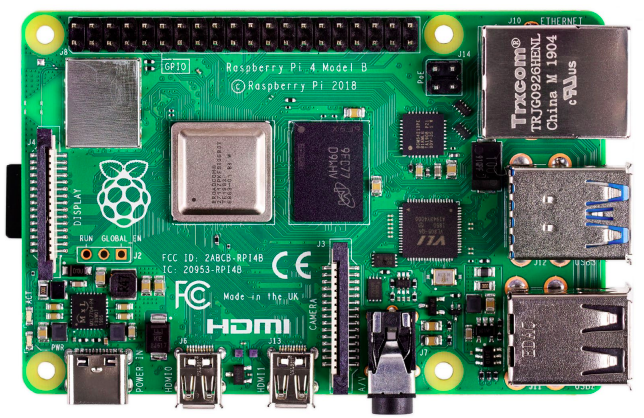
\includegraphics[width=0.6\columnwidth]{./img/raspberry.png}
  \caption{Raspberry Pi model 4B}%
\label{fig:raspberri}
\end{figure}

\subsection{Motion Detection}
\label{sec:motion-detec}

For the motion detection, it was already mentioned in section \ref{sec:motion-detection} that the best option is to use an ultrasonic sensor. Thus, the sensor that has been chosen is the \texttt{HC-SR04 Ultrasonic Sensor}. This sensor has the following specifications~\cite{sensor}:
%
\begin{item-c}
\item \emph{Operating Voltage}: 5V \gls{dc};
\item \emph{Operating Current}: 15 \gls{ma};
\item \emph{Operating Frequency}: 40 KHz;
\item \emph{Maximum Range}: 4 meters;
\item \emph{Minimum Range}: 2 centimeters;
\item \emph{Ranging Accuracy}: 3 millimeters;
\item \emph{Measuring Angle}: 15 degrees;
\item \emph{Trigger Input Signal}: 10 microseconds \gls{ttl} pulse;
\item \emph{Dimension}: 45 x 20 x 15 millimeters.
\end{item-c}

\subsubsection{Sensor Pinout}

In Fig.~\ref{fig:sensor-pinout} is described the sensor pinout and each pin works as follows~\cite{sensor}:
%
\begin{enum-c}
\item is the power supply for HC-SR04 Ultrasonic distance sensor which we connect to a 5V supply (for example, 5V pin on Raspberry);
\item pin that is used to trigger the ultrasonic sound pulses;
\item pin that produces a pulse when the reflected signal is received. The length of the pulse is proportional to the time it took for the transmitted signal to be detected.
\item pin that should be connected to the ground (for example, GND pin of the Raspberry).
\end{enum-c}
%
\begin{figure}[htb!]
\centering
    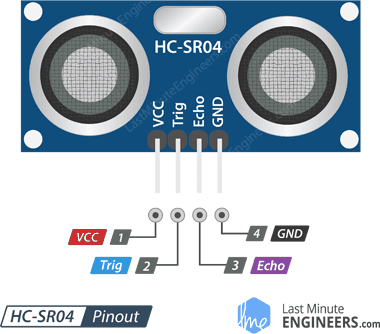
\includegraphics[width=0.4\columnwidth]{./img/sensor-pinout.png}
  \caption{HC-SR04 Pinout (withdrawn from \cite{sensor})}%
\label{fig:sensor-pinout}
\end{figure}

For this project it will be used three sensors, one placed on the bottom, another on the middle and another one on the top of the machine. 
With this setup, it can be avoided some perturbations like an animal walking in front of the machine (only the bottom sensor will detect). The disposition of the middle and top sensors can't be too high, because of short people, for example.

%\subsubsection{How does it work}
%On Fig.\ref{fig:sensor-behavior-ex} is an example on how does the sensor works.
%
%\begin{figure}[htb!]
%\centering
%    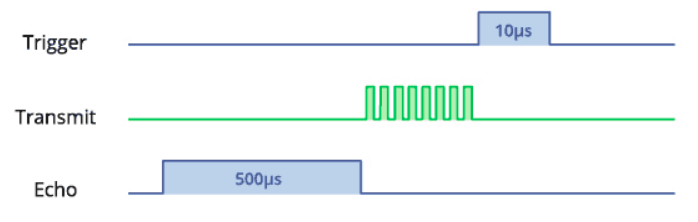
\includegraphics[width=0.6\columnwidth]{./img/sensor-behaviour-ex.png}
%  \caption{HC-SR04 behavior example (withdrawn from %\cite{sensor})}%
%\label{fig:sensor-behavior-ex}
%\end{figure}

%It all starts, when a pulse of at least 10 microseconds in duration is applied to the Trigger pin. In response to that, the sensor transmits a sonic burst of eight pulses at 40 KHz. This 8-pulse pattern makes the "ultrasonic signature" from the device unique, allowing the receiver to differentiate the transmitted pattern from the ambient ultrasonic noise~\cite{sensor}.

%The eight ultrasonic pulses travel through the air away from the transmitter. Meanwhile the Echo pin goes \texttt{HIGH} to start forming the beginning of the echo-back signal.
%In case, If those pulses are not reflected back then the Echo signal will timeout after 38 milliseconds and return \texttt{LOW}. Thus a 38 milliseconds pulse indicates no obstruction within the range of the sensor~\cite{sensor}.

%After the echo pin return low, it can be verified the distance of the obstacle to the sensor through some mathematics calculations.
%It is known that in this case \texttt{distance = time * speed}, being speed the speed of sound and time the time of the pulse.

\subsection{Fragrance Diffusion Actuator}

The chosen fragrance diffusion actuator is in Fig.~\ref{fig:fragrance-module} and has the following specifications~\cite{fragrance-module}:

It has an operating voltage of \texttt{5V \gls{dc}} and an operating current of \texttt{300 \gls{ma}}. The operating power is \texttt{2 Watt}. It has a fixed frequency single-chip microcomputer with a frequency of \texttt{108 KHz}. The dimensions of the board of the module are \texttt{35 * 20 * 17 millimeters}.
It has a \texttt{strong versatility}, large amount of fog, \texttt{stable performance}, the chip has an automatic timing shutdown function (4 hours of continuous work will automatically shut down protection, to turn on again, press the power on again). The 5V USB power supply mode, can be powered by MICRO charging cable.
The net diameter of the atomized steel sheet is 16 millimeters, the outer diameter of the silicone ring is 20 millimeters, and the wire length is 8 centimeters.
%
\begin{figure}[htb!]
\centering
    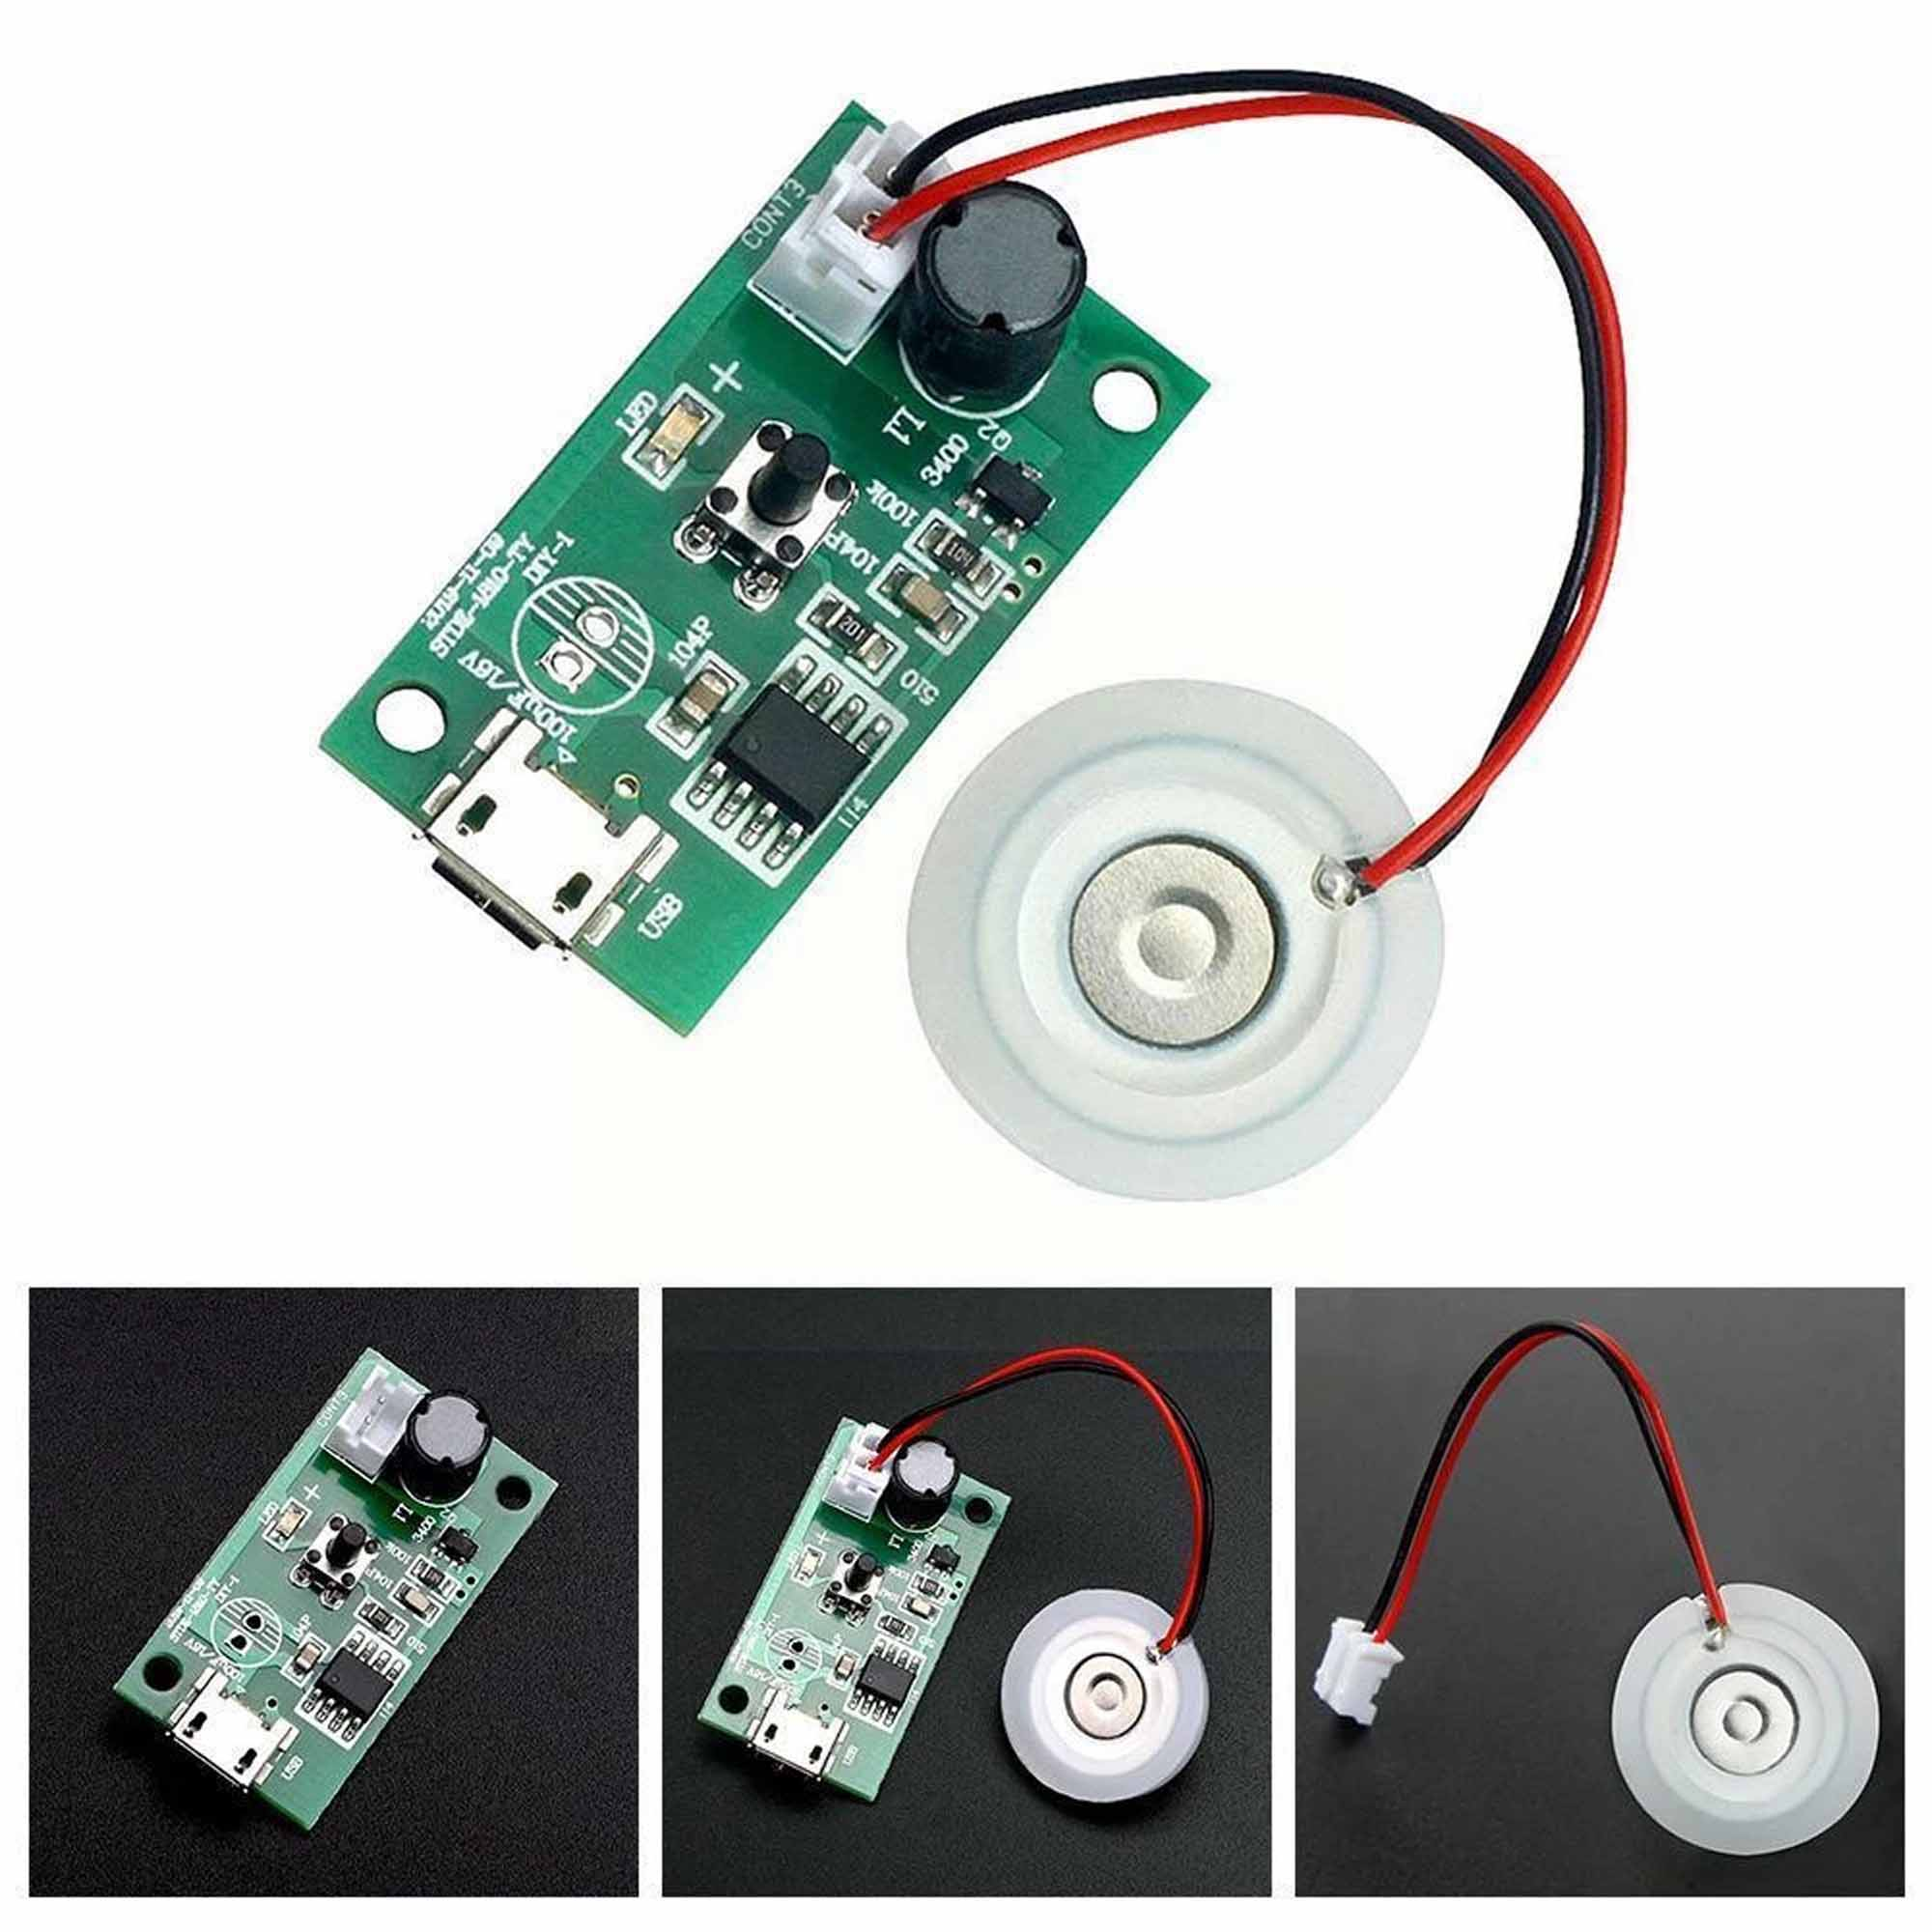
\includegraphics[width=0.5\columnwidth]{./img/fragrance-module.jpg}
  \caption{Fragrance module (withdrawn from \cite{fragrance-module})}%
\label{fig:fragrance-module}
\end{figure}


\subsection{Camera}
The camera to use in this project needs to be compatible with the board in use, in this case, the Raspberry Pi.
Thus the camera module that is used is the \texttt{Raspberry Pi Camera Module V2} (Fig.~\ref{fig:camera-module}).
%
\begin{figure}[htb!]
\centering
    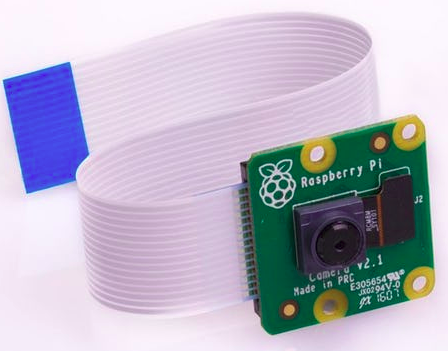
\includegraphics[width=0.4\columnwidth]{./img/camera-module.png}
  \caption{Camera module (withdrawn from \cite{camera-module})}%
\label{fig:camera-module}
\end{figure}

This camera module has a \texttt{Sony IMX219 8-megapixel sensor} and can be used to take high-definition video, as well as stills photographs. It supports 1080p30, 720p60 and VGA90 video modes, as well as still capture. It attaches via a 15 centimeters ribbon cable to the \gls{csi} port on the Raspberry Pi. The camera works with all models of Raspberry Pi 1, 2, 3 and 4. It can be accessed through the MMAL and V4L APIs, and there are numerous third-party libraries built for it, including the Picamera Python library.~\cite{camera-module}.

\subsection{LCD Display}

In Fig.~\ref{fig:screen} is the display that is used in this project. One advantage on this display is that it has \texttt{audio drivers}, which means that it is only necessary to plug a speaker and the board can handle the rest. It is also important to refer that the display isn't touch because there is no need to it and also this was the chosen one because it was the bigger and best on market considering quality and price.

As it can be seen, the display has \texttt{10.1 inches} and it is supplied with \texttt{5V \gls{dc}} and with a current of \texttt{2 A} via a micro USB port.
Fig.~\ref{fig:screen-interfaces} show all the interfaces that the board module of the display provides. That was also one more reason for the choice of this display: it has an \texttt{\gls{hdmi} interface} to connect to the Raspberry, the \texttt{50Pin TTL Screen Interface} that will connect to the display and two options to plug audio - the \texttt{Speaker Interface} and the \texttt{3.5mm audio interface}.
%
\begin{figure}[htb!]
\centering
    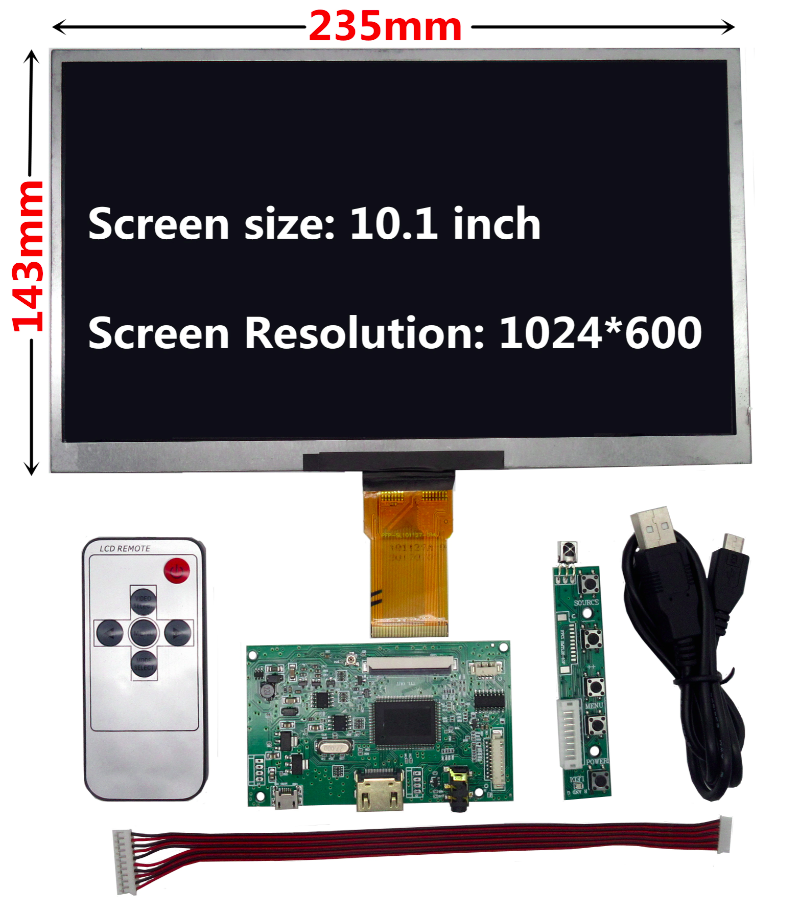
\includegraphics[width=0.4\columnwidth]{./img/screen.png}
  \caption{Display (withdrawn from \cite{screen})}%
\label{fig:screen}
\end{figure}
%
\begin{figure}[htb!]
\centering
    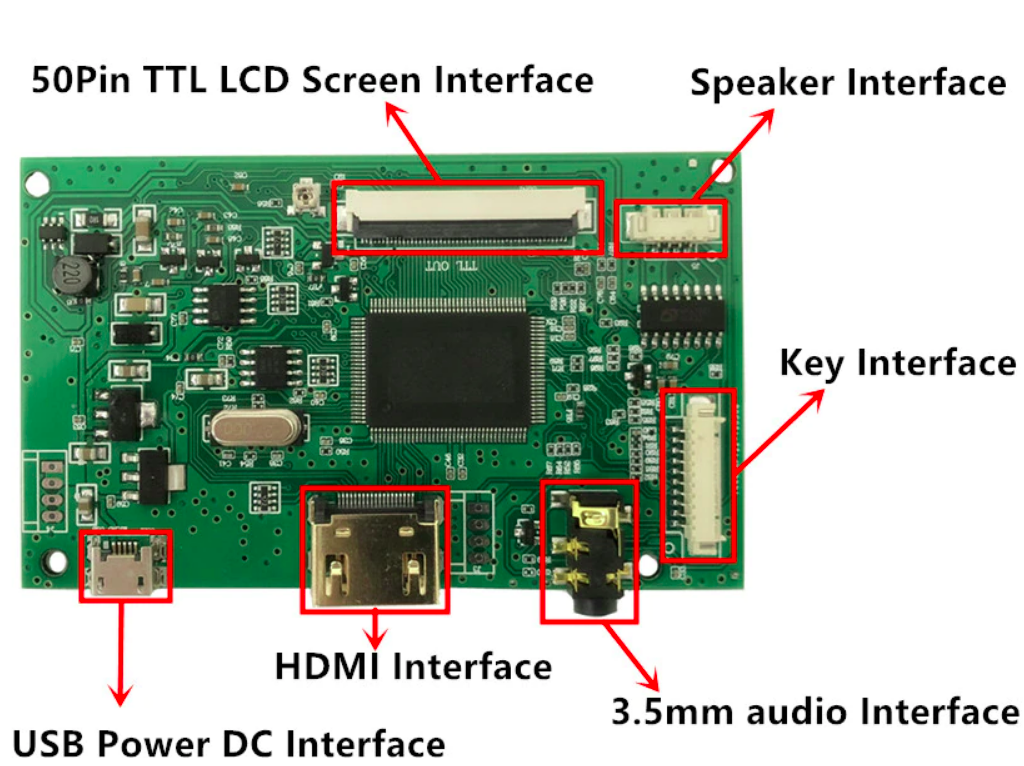
\includegraphics[width=0.6\columnwidth]{./img/screen-interfaces.png}
  \caption{Display Interfaces (withdrawn from \cite{screen})}%
\label{fig:screen-interfaces}
\end{figure}

It can also be seen in this figure that the display has also a remote and a board to handle the remote controls, but in this implementation, it will probably not be in use.

\subsection{Speakers}
When playing video ads, it is not only necessary a display, but also a speaker to playback the sound of the ads.
As it can be seen in Fig.~\ref{fig:screen-interfaces}, the screen board has two different interfaces of audio: the speaker interface and the audio interface.
For this project it will be used speakers that uses the speaker interface, because that type of speakers with that interface are passive speakers and don't need a \gls{dc} power supply, which is an advantage~\cite{passive-speaker}.

Thus, the speakers that will be used have an impedance of \texttt{8 Ohm} and a power of \texttt{5 Watts} and are displayed on Fig~\ref{fig:speakers}.
%
\begin{figure}[htb!]
\centering
    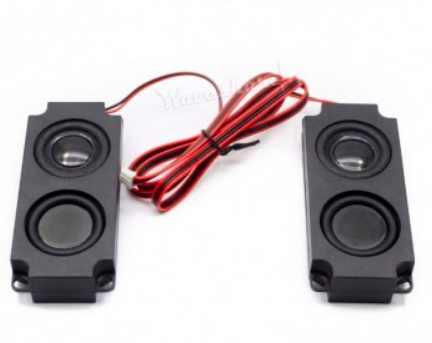
\includegraphics[width=0.4\columnwidth]{./img/speakers.png}
  \caption{Speakers (withdrawn from \cite{speakers})}%
\label{fig:speakers}
\end{figure}

\subsection{Power Supply}

The \gls{mdo-l} will be a plugged in system, so it will be needed a plugged in power supply to supply all the components of the system. In total, the power consumption will not overtake 20 Watts and all the supplies necessary are plugged by USB (Raspberry Pi, Fragrance Diffusion Actuator, and screen). So, it will be used the power supply in Fig.~\ref{fig:power-supply}, that has 4 outputs of \texttt{5 V \gls{dc}} and \texttt{2.4 A \gls{dc}} each.
%
\begin{figure}[htb!]
\centering
    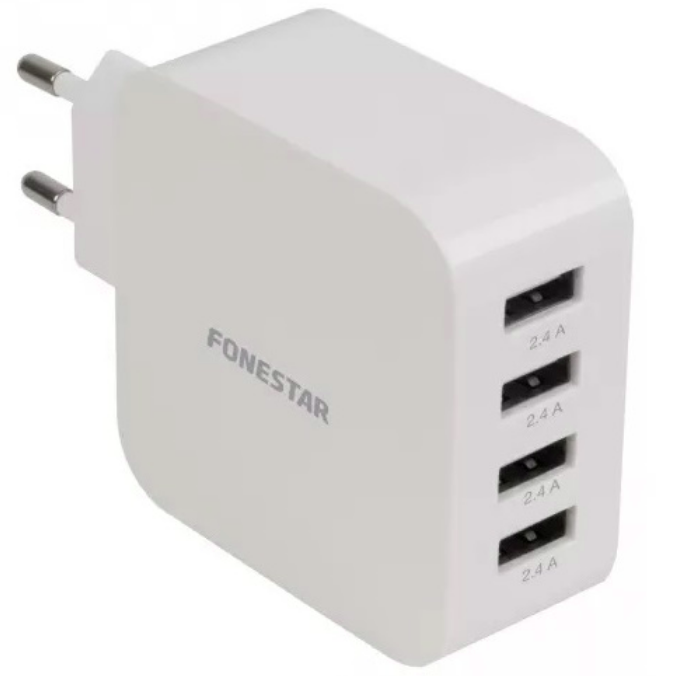
\includegraphics[width=0.3\columnwidth]{./img/power-supply.png}
  \caption{Power Supply (withdrawn from \cite{power-supply})}%
\label{fig:power-supply}
\end{figure}

\subsection{Total \gls{hw} cost}

The total cost can now be precisely calculated, once that all the hardware is now specified on table \ref{tab:hw-costs}.

% Please add the following required packages to your document preamble:
\begingroup
\renewcommand{\arraystretch}{0.7} % Default value: 1
% Please add the following required packages to your document preamble:
% \usepackage{booktabs}
% \usepackage{graphicx}
\begin{table}[]
\centering
\caption{Total spending on Hardware}
\label{tab:hw-costs}
\resizebox{\textwidth}{!}{%
\begin{tabular}{@{}lll@{}}
\toprule
\textbf{Item}                & \textbf{Quantity} & \textbf{Price (€)} \\ \midrule
Raspberry Pi 4B              & 1                 & 70.00              \\ \midrule
Ultrasonic Sensor HC-SR04    & 3                 & 11.70              \\ \midrule
Fragrance Diffusion Actuator & 1                 & 3.23               \\ \midrule
Raspberry Pi Camera V2       & 1                 & 20.00              \\ \midrule
LCD Display                  & 1                 & 51.95              \\ \midrule
Speakers                     & 1                 & 3.00               \\ \midrule
Power Supply                 & 1                 & 13.50              \\ \midrule
\multicolumn{2}{l}{\textbf{Total}}               & \textbf{173.38}    \\ \bottomrule
\end{tabular}%
}
\end{table}
% components. Fig.~\ref{fig:block-diag} depicts the overall information flow and
% the TV remote block diagram: the \texttt{User} interacts with
% the TV remote by pressing buttons which triggers the emission of \gls{ir} codes
% to the TV, containing the \gls{ir} receiver. As supported by the market research
% seen in
% Section~\ref{sec:market-research}, the block diagram of the TV remote control
% can be taught of a physical input interface --- the pushbuttons, a processing
% interface --- a microprocessor --- to determine which keys are pressed and the
% resulting \gls{ir} codes to be emitted, and a \gls{ir} transmitter circuit as
% the output where the IR LED also works as a visual output. Usually, there will
% be also a digital interface, to handle the large amount of keys as a
% \gls{io} expander with serial interface, e.g. the Microchip MCP23008/MCP23S08~\cite{microchip}, which is considered here for future expansibility of the device,
% thus making it scalable. This can be especially useful when using
% microprocessor units with lower I/O inputs. A tradeoff between the inclusion of
% the multiplexer versus future redesign must be performed. The system is powered
% by batteries.
% 
% The microprocessor chosen depends on various factors, such as: architecture,
% throughput, memory, processing power, power efficiency, toolchain availability
% and programming easiness, etc. Additionally, one may consider the usage of a
% microcontroller, due to added peripherals, easing the \gls{sw} burden. For
% example, the usage of the \gls{pca} peripheral in the 8051 \gls{mcu} can free the processor from the
% job of bit-banging the IR transmitter circuitry or the \gls{i2c} or \gls{spi} peripherals to
% interface the I/O expander. With that said, the choice
% relied on the 8051 MCU due to its small footprint, clock speed of up to 48 MHz,
% low power usage on idle, the acquaintance with the toolchain and the
% programming, and for the inclusion of the PCA, SPI and I2C peripherals.  
% %
%   \vspace{-5mm}
% %  
% %- Block diagram with COTS components, if possible
% %- List of constraints of functions to be implemented in HW or SW
% %  - Inclusion of a multiplexer may reduce SW burden
% %  - CPU peripherals:
% %  - PCA for wave generation
% %  
% \begin{figure}[htb!]
% \centering
%     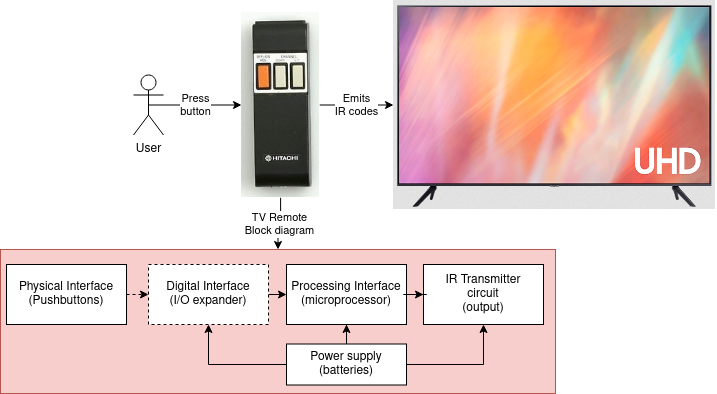
\includegraphics[width=0.7\columnwidth]{./img/block-diagram.png}
%   \caption{Overall information flow and TV remote block diagram}%
% \label{fig:block-diag}
% \end{figure}
% %
%   \vspace{-5mm}
% %  
\section{Hardware interfaces definition}
\label{sec:hw-interf-def}
% After specifying the \gls{hw}, it is important to define its interfaces. The
% TV remote control is clearly an event-driven asynchronous system, thus using HW
% interrupts. When a user presses a pushbutton that event should be signaled to
% the \gls{cpu} of the MCU via an external interrupt, ``waking'' it up. The CPU
% handles that interrupt via an \gls{isr}, processing it and actuating, if
% required. The system then goes back to sleep.
% 
% The 8051 MCU only contains 2 external interrupts sources --- \texttt{INTO} and
% \texttt{INT1} --- thus limitting the direct connection of the pushbuttons to the
% MCU, even with the pull-up circuitry. This is where the serial I/O expander
% becomes most useful, as it can be connected to TV remote keys (up to 8 in this
% case) and connected to a single external interrupt pin, being then read via
% \gls{i2c} or \gls{spi} interface. Thus, the keys can be connected through
% pull-up circuitry to the I/O expander and the output is then connected to
% \texttt{INTO} on the 8051 MCU. The communication protocol chosen is \gls{i2c} as
% it is more expandable
% 
% Concerning the output, the 8051 PCA peripheral is connected to the IR
% transmitter circuitry, for IR code emission. The HW interfaces of the system are
% depicted in Fig.~\ref{fig:hw-interfaces}.
% %
%   \vspace{-5mm}
% %  
% \begin{figure}[htb!]
% \centering
%     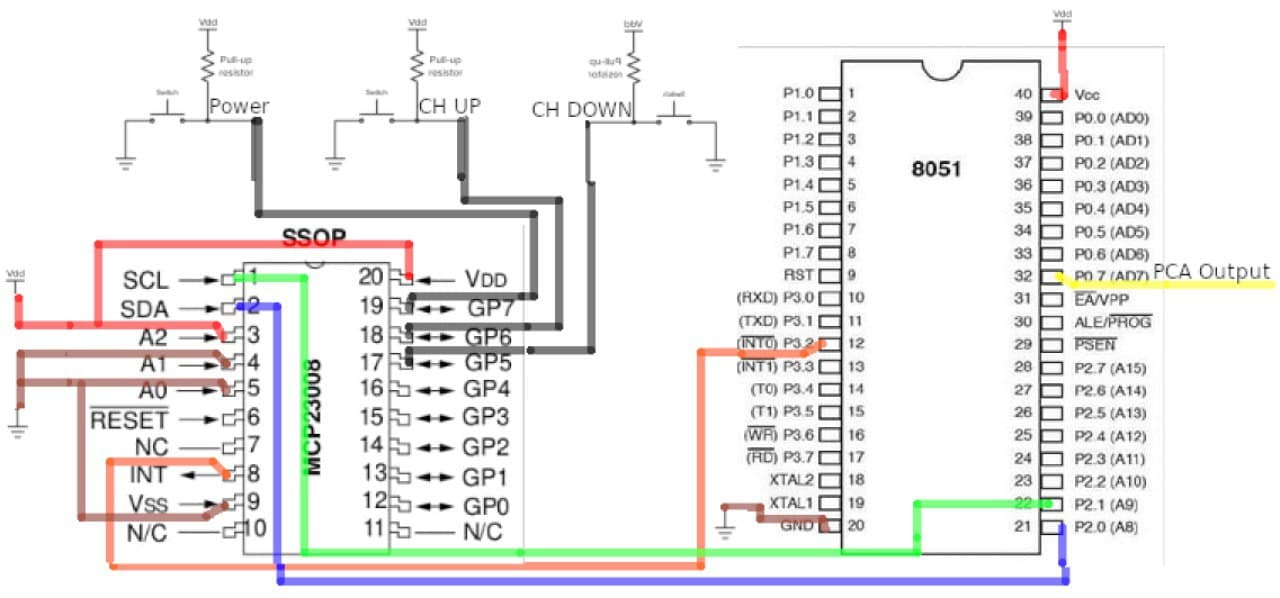
\includegraphics[width=1.0\columnwidth]{./img/hw-interfaces.jpg}
%   \caption{HW interfaces of the system}%
% \label{fig:hw-interfaces}
% \end{figure}
% %
% %
%   \vspace{-5mm}
%  
%%% Local Variables:
%%% mode: latex
%%% TeX-master: "../../../dissertation"
%%% End:
